\chapter[Rubidium Production in Massive AGB Stars]{\textbf{Rubidium Production in \\ Massive AGB Stars}}
\label{ch:Rb}

% \cite{Iliadis2020} for mutual information (and the original 1950's paper)

% In some cases, the MACS of radioactive nuclei can be measured by the activation technique (Ref. Kappeler 2011), because of the ability to use extremely small sample masses. Howerver, measurements of the MACS for the branch point at $^{85}$Kr is hampered by the high specific activity. (The data obtained via activation usually represent the respective MACS values at kT = 25 keV and have to be extrapolated to higher and lower temperatures by means of theoretical data)

\section{Introduction}

% Chapter \ref{ch:Rb} will address the ``rubidium problem'' in massive AGB stars, a descrepancy between observed and theoretical rubidium abundances from s-process nucleosynthesis. The s-process branching at $^{86}$Rb is investigated through a Monte Carlo reaction network approach, identifying the most important reactions to rubidium abundance.
%The measurements of the $^{86}\mathrm{Kr}(^{3}\mathrm{He},d)^{87}\mathrm{Rb}$ transfer reaction and the $^{87}\mathrm{Rb}(\gamma,\gamma')^{87}\mathrm{Rb}$ and $^{87}\mathrm{Rb}(\gamma,n)^{86}\mathrm{Rb}$ photoabsorption reactions are proposed to enhance our understanding of the closed-N shell nucleus $^{87}$Rb and its involvement in the rubidium overabundance. 

This chapter details the investigation of the s-process branching at $^{86}$Rb to identify the key reaction rates constraining rubidium production in massive AGB stars. Section \ref{sec:Rb_Abundance} will introduce the ``rubidium problem'', a discrepancy between the observed and theoretical [Rb/Zr] abundance ratios of massive AGB stars. Section \ref{sec:network_method} will describe the reaction network methodology used in the present work for investigating the s-process branching at $^{86}$Rb. The results of a single network calculation are presented, and the extension to a Monte Carlo reaction network procedure is described. Section \ref{sec:rate_sensitivities} showcases the results of the Monte Carlo reaction network calculation, where the effects of reaction rate uncertainties on rubidium abundance are demonstrated. The reactions with the strongest correlation to the $^{87}\mathrm{Rb}/^{86}\mathrm{Sr}$ and $^{87}\mathrm{Rb}/^{90}\mathrm{Zr}$ abundance ratios are reported. Finally, Section \ref{sec:86Rb_n_g_rate} details the most recent reaction rate constraint of $^{86}\mathrm{Rb}(n,\gamma)^{87}\mathrm{Rb}$, found to be one of the most important reactions for rudibium production in this work.

\section{Rubidium Abundance} \label{sec:Rb_Abundance}

% Show the Kr - Rb s-process path

% Significant overabundance (predicted vs. observed solar system abundance) of Rb, even accounting for r-process contribution(?).

% 22Ne(a,n)25Mg reaction rate should be sensitive to the Sr/Rb abundance ratio

% Theoretical motivation for 86Rb(n,g)87Rb measurement... (but the real motivation is the RESULT of my sensitivity study of the predicted Rb/Sr abundance ratio with respect to the 22Ne(a,n)25Mg neutron source)

% P1: Introduction and recap of AGB neutron sources

Asymptotic giant branch (AGB) stars of sufficient mass ($M \gtrsim 4$ $M_{\odot}$) initiate hot-bottom burning (HBB; see Section \ref{sec:hot-bottom-burning}) as a result of the increased temperatures at the bottom of the convective hydrogen envelope. Between thermal pulses, $^{12}$C is destroyed by proton-capture reactions during the sequence $^{12}\mathrm{C}(p,\gamma)^{13}\mathrm{N}(\beta^{+}\nu)^{13}\mathrm{C}(p,\gamma)^{14}\mathrm{N}$. This effect is observed in massive AGB stars due to the decreased C/O ratio, and the most massive stars become O-rich, despite the dredge-up of C during third drege-up (3DUP) events \cite{Garcia2006}. The sequence also forms both a $^{13}$C pocket and a $^{14}$N pocket at the top of the He-rich intershell region, even in the absence of HBB through proton mixing. During thermal pulses, $^{14}$N captures $\alpha$-particles via the sequence $^{14}\mathrm{N}(\alpha,\gamma)^{18}\mathrm{F}(\beta^{+}\nu)^{18}\mathrm{O}(\alpha,\gamma)^{22}\mathrm{Ne}$. The two reactions $^{13}\mathrm{C}(\alpha,n)^{16}\mathrm{O}$ and $^{22}\mathrm{Ne}(\alpha,n)^{25}\mathrm{Mg}$ are the predominant sources of free neutrons in the intershell region, occuring during the interpulse period and during thermal pulses, respectively. The $^{13}\mathrm{C}(\alpha,n)^{16}\mathrm{O}$ reaction is the main neutron source for low and intermediate-mass AGB stars ($\lesssim 4$ $M_{\odot}$), where neutron densities are $N_{n} \approx 10^{7}$ $\mathrm{g}/\mathrm{cm}^{3}$. Meanwhile, the $^{22}\mathrm{Ne}(\alpha,n)^{25}\mathrm{Mg}$ reaction is expected to dominate for massive AGB stars, where neutron densities reach $N_{n} \approx 10^{10}$ $\mathrm{g}/\mathrm{cm}^{3}$. The free neutrons lead to nucleosynthesis of heavy elements such as Rb, Sr, Y, and Zr via the s-process (see Section \ref{sec:s-process}). These elements are brought to the surface during subsequent 3DUP events and are ejected into the interstellar medium. 

\subsection{The s-Process Branching at $^{86}$Rb} \label{subsec:86Rb_Branch}

The $^{22}\mathrm{Ne}(\alpha,n)^{25}\mathrm{Mg}$ neutron source enhances the efficiency of s-process branchings, altering the relative abundance of nearby nuclei. Hence, the abundance ratio of nuclei before and after an s-process branching is an indicator of both the neutron density and the predominant neutron source \cite{Garcia2006}. The branchings at $^{85}$Kr and $^{86}$Rb, for example, determine whether the production of the closed-neutron shell ($N=50$) nucleus $^{87}$Rb is favored. This situation is depicted in Figure \ref{fig:Rb86Branch}, where stable nuclei are shaded, and unstable nuclei are unshaded. The $^{85}$Kr and $^{86}$Rb s-process branchings are highlighted in red, and their corresponding neutron captures or $\beta^{-}$-decays are illustrated with dashed arrows. A complication arises with $^{85}$Kr, since the $^{84}\mathrm{Kr}(n,\gamma)^{85}\mathrm{Kr}$ reaction can populate the $^{85}\mathrm{Kr}^{m}$ isomeric state at roughly equal probability to that of the $^{85}\mathrm{Kr}^{g}$ ground state \cite{Raut2013}. The $^{85}\mathrm{Kr}^{m}$ state $\beta^{-}$-decays to $^{85}$Rb with about an $80\%$ probability. Otherwise, it $\gamma$-decays to the ground state with about a $20\%$ probability. Only the ground state can undergo neutron capture. In the absense of large neutron densities, $^{85}$Kr and $^{86}$Rb will preferrentially $\beta^{-}$-decay, bypassing $^{87}$Rb altogether. If, on the other hand, there is a sufficiently large neutron density from the $^{22}\mathrm{Ne}(\alpha,n)^{25}\mathrm{Mg}$ neutron source, $^{87}$Rb will be accumulated. Since $^{87}$Rb is a closed-shell nucleus, it also has an exceptionally low neutron-capture cross section, increasing its abundance even more. In this latter scenario, we should expect $^{87}$Rb to be much more abundant than, say, $^{86}$Sr or $^{90}$Zr.

\def\BoxSpace{0.3} % Defining the variable BoxSpace to value in brackets
\def\BoxSpacetwo{\BoxSpace * 2} % So I don't have to keep doing {2+(\BoxSpace * 2)}
\def\BoxSpacethree{\BoxSpace * 3}
\def\BoxSpacefour{\BoxSpace * 4}
\def\BoxSpacehalf{\BoxSpace * 0.5}
\def\AOS{0.1} % Arrow Offset
\def\AW{0.52} % Arrow Width (mm)

\begin{figure}[t]
\centering
\begin{tikzpicture}[scale=2.0, every node/.style={transform shape}]

% (0,0) is at the bottom left corner of plot, where 84Kr is.
\filldraw[fill = light-gray] (0,0) rectangle (1,1); % 84Kr box
\draw (1+\BoxSpace,0) rectangle (2+\BoxSpace,1); %85Kr box
\filldraw[fill = light-gray] (2+\BoxSpacetwo,0) rectangle (3+\BoxSpacetwo,1); % 86Kr box
\draw (3+\BoxSpacethree,0) rectangle (4+\BoxSpacethree,1); %87Kr box
\filldraw[fill = light-gray] (0,1+\BoxSpace) rectangle (1,2+\BoxSpace); % 85Rb box
\draw (1+\BoxSpace,1+\BoxSpace) rectangle (2+\BoxSpace,2+\BoxSpace); %86Rb box
\filldraw[fill = light-gray] (2+\BoxSpacetwo,1+\BoxSpace) rectangle (3+\BoxSpacetwo,2+\BoxSpace); % 87Rb box
\draw (3+\BoxSpacethree,1+\BoxSpace) rectangle (4+\BoxSpacethree,2+\BoxSpace); %88Rb box

\filldraw[fill = light-gray] (0,2+\BoxSpacetwo) rectangle (1,3+\BoxSpacetwo); % 86Sr box
\filldraw[fill = light-gray] (1+\BoxSpace,2+\BoxSpacetwo) rectangle (2+\BoxSpace,3+\BoxSpacetwo); %87Sr box
\filldraw[fill = light-gray] (2+\BoxSpacetwo,2+\BoxSpacetwo) rectangle (3+\BoxSpacetwo,3+\BoxSpacetwo); % 88Sr box
\draw (3+\BoxSpacethree,2+\BoxSpacetwo) rectangle (4+\BoxSpacethree,3+\BoxSpacetwo); %89Sr box

\filldraw[fill = light-gray] (2+\BoxSpacetwo,3+\BoxSpacethree) rectangle (3+\BoxSpacetwo,4+\BoxSpacethree); % 89Y box
\draw (3+\BoxSpacethree,3+\BoxSpacethree) rectangle (4+\BoxSpacethree,4+\BoxSpacethree); % 90Y box
\filldraw[fill = light-gray] (2+\BoxSpacetwo,4+\BoxSpacefour) rectangle (3+\BoxSpacetwo,5+\BoxSpacefour); % 90Zr box
\filldraw[fill = light-gray] (3+\BoxSpacethree,4+\BoxSpacefour) rectangle (4+\BoxSpacethree,5+\BoxSpacefour); % 91Zr box

\node at (0.5,0.5) {\footnotesize{$^{84}\mathrm{Kr}$}};
\node[text=black!20!red] at (1+\BoxSpace+0.5,0.5) {\footnotesize{$^{85}\mathrm{Kr}$}};
\node at (2+\BoxSpacetwo+0.5,0.5) {\footnotesize{$^{86}\mathrm{Kr}$}};
\node at (3+\BoxSpacethree+0.5,0.5) {\footnotesize{$^{87}\mathrm{Kr}$}};
\node at (0.5,1+\BoxSpace+0.5) {\footnotesize{$^{85}\mathrm{Rb}$}};
\node[text=black!20!red] at (1+\BoxSpace+0.5,1+\BoxSpace+0.5) {\footnotesize{$^{86}\mathrm{Rb}$}};
\node at (2+\BoxSpacetwo+0.5,1+\BoxSpace+0.5) {\footnotesize{$^{87}\mathrm{Rb}$}};
\node at (3+\BoxSpacethree+0.5,1+\BoxSpace+0.5) {\footnotesize{$^{88}\mathrm{Rb}$}};
\node at (0.5,2+\BoxSpacetwo+0.5) {\footnotesize{$^{86}\mathrm{Sr}$}};
\node at (1+\BoxSpace+0.5,2+\BoxSpacetwo+0.5) {\footnotesize{$^{87}\mathrm{Sr}$}};
\node at (2+\BoxSpacetwo+0.5,2+\BoxSpacetwo+0.5) {\footnotesize{$^{88}\mathrm{Sr}$}};
\node at (3+\BoxSpacethree+0.5,2+\BoxSpacetwo+0.5) {\footnotesize{$^{89}\mathrm{Sr}$}};
\node at (2+\BoxSpacetwo+0.5,3+\BoxSpacethree+0.5) {\footnotesize{$^{89}\mathrm{Y}$}};
\node at (3+\BoxSpacethree+0.5,3+\BoxSpacethree+0.5) {\footnotesize{$^{90}\mathrm{Y}$}};
\node at (2+\BoxSpacetwo+0.5,4+\BoxSpacefour+0.5) {\footnotesize{$^{90}\mathrm{Zr}$}};
\node at (3+\BoxSpacethree+0.5,4+\BoxSpacefour+0.5) {\footnotesize{$^{91}\mathrm{Zr}$}};

\draw[line width = \AW mm, -{Triangle[]}] (1-\AOS,0.5) -- (1+\BoxSpace+\AOS, 0.5); % 84Kr(n,g)
\draw[line width = \AW mm, -{Triangle[]},dashed] (2+\BoxSpace-\AOS,0.5) -- (2+\BoxSpacetwo+\AOS,0.5); % 85Kr(n,g)
\draw[line width = \AW mm, -{Triangle[]}] (3+\BoxSpacetwo-\AOS,0.5) -- (3+\BoxSpacethree+\AOS, 0.5); % 86Kr(n,g)
\draw[line width = \AW mm, -{Triangle[]},dashed] (1+\BoxSpace+\AOS,1-\AOS) -- (1-\AOS,1+\BoxSpace+\AOS); % 85Kr(g,g)
\draw[line width = \AW mm, -{Triangle[]}] (3+\BoxSpacethree+\AOS,1-\AOS) -- (3+\BoxSpacetwo-\AOS,1+\BoxSpace+\AOS); % 87Kr(g,g)
\draw[line width = \AW mm, -{Triangle[]}] (1-\AOS,1+\BoxSpace+0.5) -- (1+\BoxSpace+\AOS,1+\BoxSpace+0.5); % 85Rb(n,g)
\draw[line width = \AW mm, -{Triangle[]},dashed] (2+\BoxSpace-\AOS,1+\BoxSpace+0.5) -- (2+\BoxSpacetwo+\AOS,1+\BoxSpace+0.5); % 86Rb(n,g)
\draw[line width = \AW mm, -{Triangle[]}] (3+\BoxSpacetwo-\AOS,1+\BoxSpace+0.5) -- (3+\BoxSpacethree+\AOS,1+\BoxSpace+0.5); % 87Rb(n,g)
\draw[line width = \AW mm, -{Triangle[]},dashed] (1+\BoxSpace+\AOS,2+\BoxSpace-\AOS) -- (1-\AOS,2+\BoxSpacetwo+\AOS); % 86Rb(g,g)
\draw[line width = \AW mm, -{Triangle[]}] (3+\BoxSpacethree+\AOS,2+\BoxSpace-\AOS) -- (3+\BoxSpacetwo-\AOS,2+\BoxSpacetwo+\AOS); % 88Rb(g,g)
\draw[line width = \AW mm, -{Triangle[]}] (1-\AOS,2+\BoxSpacetwo+0.5) -- (1+\BoxSpace+\AOS,2+\BoxSpacetwo+0.5); % 86Sr(n,g)
\draw[line width = \AW mm, -{Triangle[]}] (2+\BoxSpace-\AOS,2+\BoxSpacetwo+0.5) -- (2+\BoxSpacetwo+\AOS,2+\BoxSpacetwo+0.5); % 87Sr(n,g)
\draw[line width = \AW mm, -{Triangle[]}] (3+\BoxSpacetwo-\AOS,2+\BoxSpacetwo+0.5) -- (3+\BoxSpacethree+\AOS,2+\BoxSpacetwo+0.5); % 88Sr(n,g)
\draw[line width = \AW mm, -{Triangle[]}] (3+\BoxSpacethree+\AOS,3+\BoxSpacetwo-\AOS) -- (3+\BoxSpacetwo-\AOS,3+\BoxSpacethree+\AOS); % 89Sr(g,g)
\draw[line width = \AW mm, -{Triangle[]}] (3+\BoxSpacetwo-\AOS,3+\BoxSpacethree+0.5) -- (3+\BoxSpacethree+\AOS,3+\BoxSpacethree+0.5); % 89Y(n,g)
\draw[line width = \AW mm, -{Triangle[]}] (3+\BoxSpacethree+\AOS,4+\BoxSpacethree-\AOS) -- (3+\BoxSpacetwo-\AOS,4+\BoxSpacefour+\AOS); % 90Y(g,g)
\draw[line width = \AW mm, -{Triangle[]}] (3+\BoxSpacetwo-\AOS,4+\BoxSpacefour+0.5) -- (3+\BoxSpacethree+\AOS,4+\BoxSpacefour+0.5); % 90Zr(n,g)
\draw[line width = \AW mm, -{Triangle[]}] (4+\BoxSpacethree-\AOS,4+\BoxSpacefour+0.5) -- (4+\BoxSpacefour+\AOS, 4+\BoxSpacefour+0.5); % 91Zr(n,g)

\node at (1+\BoxSpace+0.15,1+\BoxSpacehalf) {\tiny{g,m}}; % g = ground, m = isomeric
\node at (2+\BoxSpace+\BoxSpacehalf,0.6) {\tiny{g}};
%\node at (1+\BoxSpace+0.8,0.65) {\tiny{m}};
%\node at (1+\BoxSpace+0.8,0.35) {\tiny{g}};
%\draw[line width = \AW mm, -{Triangle[]}] (1+\BoxSpace+0.7,0.7) -- (1+\BoxSpace+0.7,0.3); % 85Kr isomeric to ground transition

\draw[dashed, line width = 0.002mm, opacity=0.4] (2+\BoxSpacetwo+0.5, -\BoxSpace) -- (3.75-\BoxSpacetwo, 5+\BoxSpacefour+\BoxSpace);
\node at (2+\BoxSpacetwo+0.5, -\BoxSpace-\BoxSpacehalf) {\scriptsize{$N = 50$}};

\end{tikzpicture}
\caption{\label{fig:Rb86Branch}The $^{85}$Kr and $^{86}$Rb s-process branchings, highlighted in red, along the s-process path from Kr to Zr. The dashed arrows extending from these branchings indicate the path dependence on the neutron density. The $N=50$ closed-shell nuclei are represented by the vertical dashed line, which have low neutron-capture cross sections. The relative abundance of $^{87}$Rb to nearby nuclei such as $^{86}$Sr and $^{90}$Zr is expected to be an indicator of neutron density.}
\end{figure}

\subsection{The Rubidium Problem} \label{subsec:Rb_Problem}

% P2: Garcia-Hernandez et al. 2006 --> Strong Rb overabundances observed in galatic O-rich massive AGB stars, coupled with a lack of strong Zr enhancements in the same stars. Not predicted by the theoretical models at the time.



% P3: Perez-Mesa et al. 2017 --> Updated observation models, but the high [Rb/Zr] observations still not reproduced by models, even ones with fine-tuned parameters, like the delayed superwind.

%The maximum observed [Rb/Fe] value at 1.3 can be reproduced by the AGB models, but the observed [Rb/Zr] values between 0.52 dex and 1.05 are not reproduced by the models.



\begin{figure}[t]
\centering
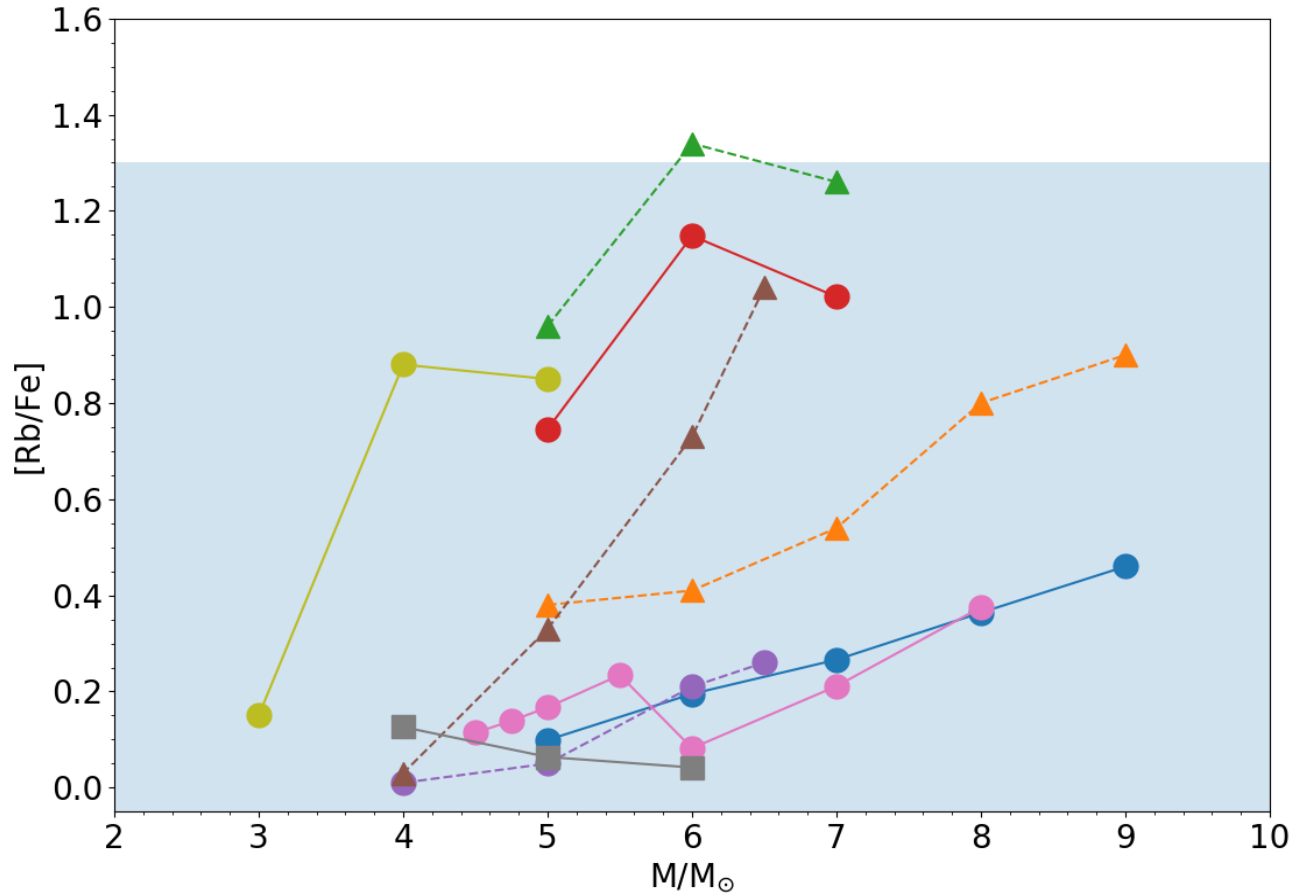
\includegraphics[width=5.0in]{Chapter-3/figs/RbProblem1.png}
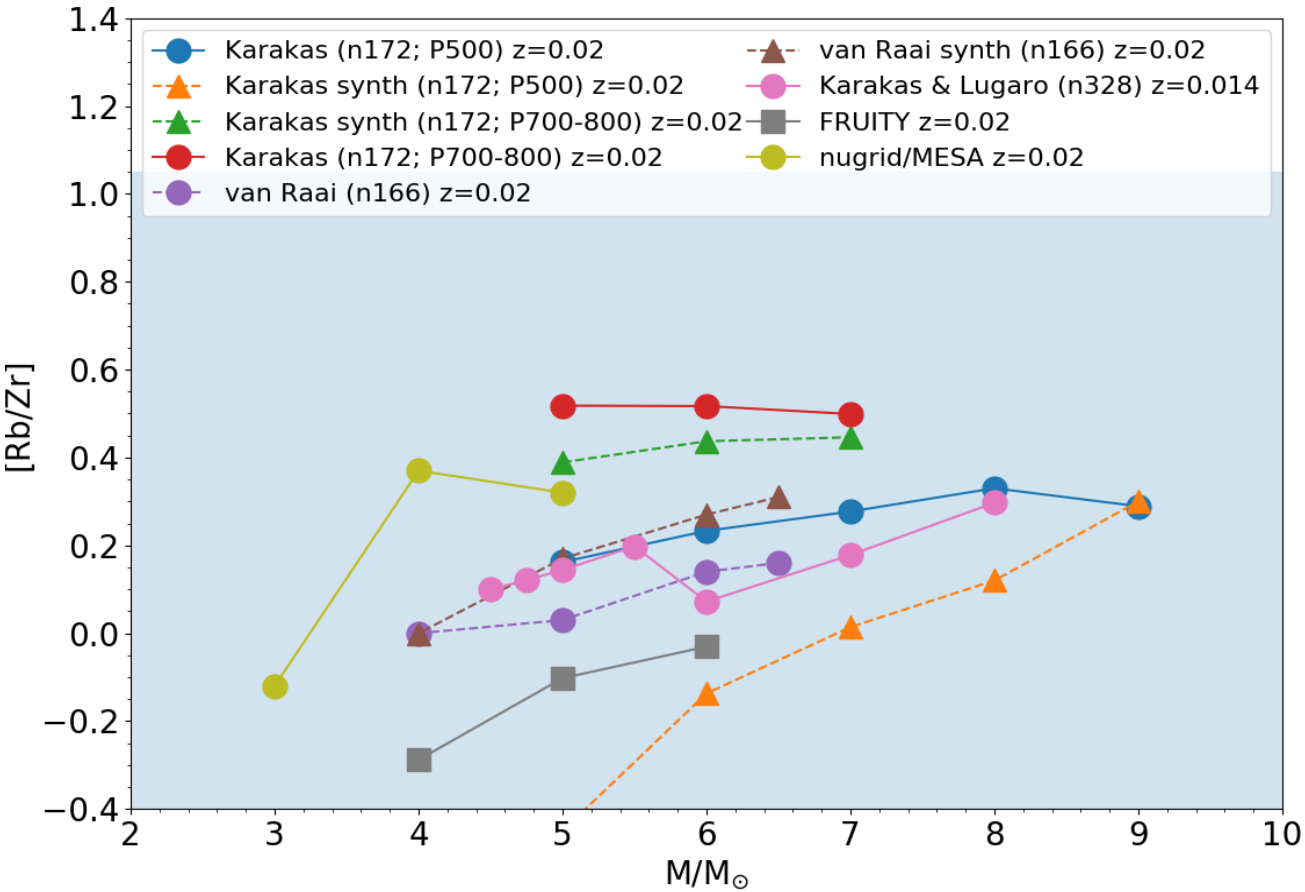
\includegraphics[width=5.0in]{Chapter-3/figs/RbProblem2.png}
\caption{\label{fig:RbProblem}The AGB model predictions of [Rb/Fe] (top) and [Rb/Zr] (bottom) as a function of stellar mass from Refs. \cite{Karakas2012,van2012,Karakas2016,Pignatari2016}. The dots and triangles represent abundances from the last computed thermal pulse and from synthetic calculations, respectively. The number of nuclei $n$ in the corresponding network is provided in the legend, as well as the delay superwind parameter $P$ (see text), if applicable, and the metallicity $z$. The range of observed [Rb/Fe] and [Rb/Zr] values from Ref. \cite{Perez2017} are shown by the shaded blue background. Adapted from Ref. \cite{Perez2017}.}
\end{figure}

\section{s-Process Reaction Network Methodology} \label{sec:network_method}



\subsection{The Reaction Network} \label{subsec:the_reaction_network}

% Description of the nuclei / reactions in the network (rates from Starlib) and their initial abundances.
% Start off with the simple 47.5% 22Ne, 47.5% 4He, and 5% 85Rb case.
% Then then solar system abundances case, where 1H --> 4He and 12C+13C --> 14N

\subsection{Abundance Evolution}

% Abundance evolution plots of 87Rb, 88Sr, Kr isotopes, 4He, 14N, 13C, etc.

\begin{figure}[t]
\begin{tikzpicture}[scale=1.0, every node/.style={transform shape}]
\node at (0,0) {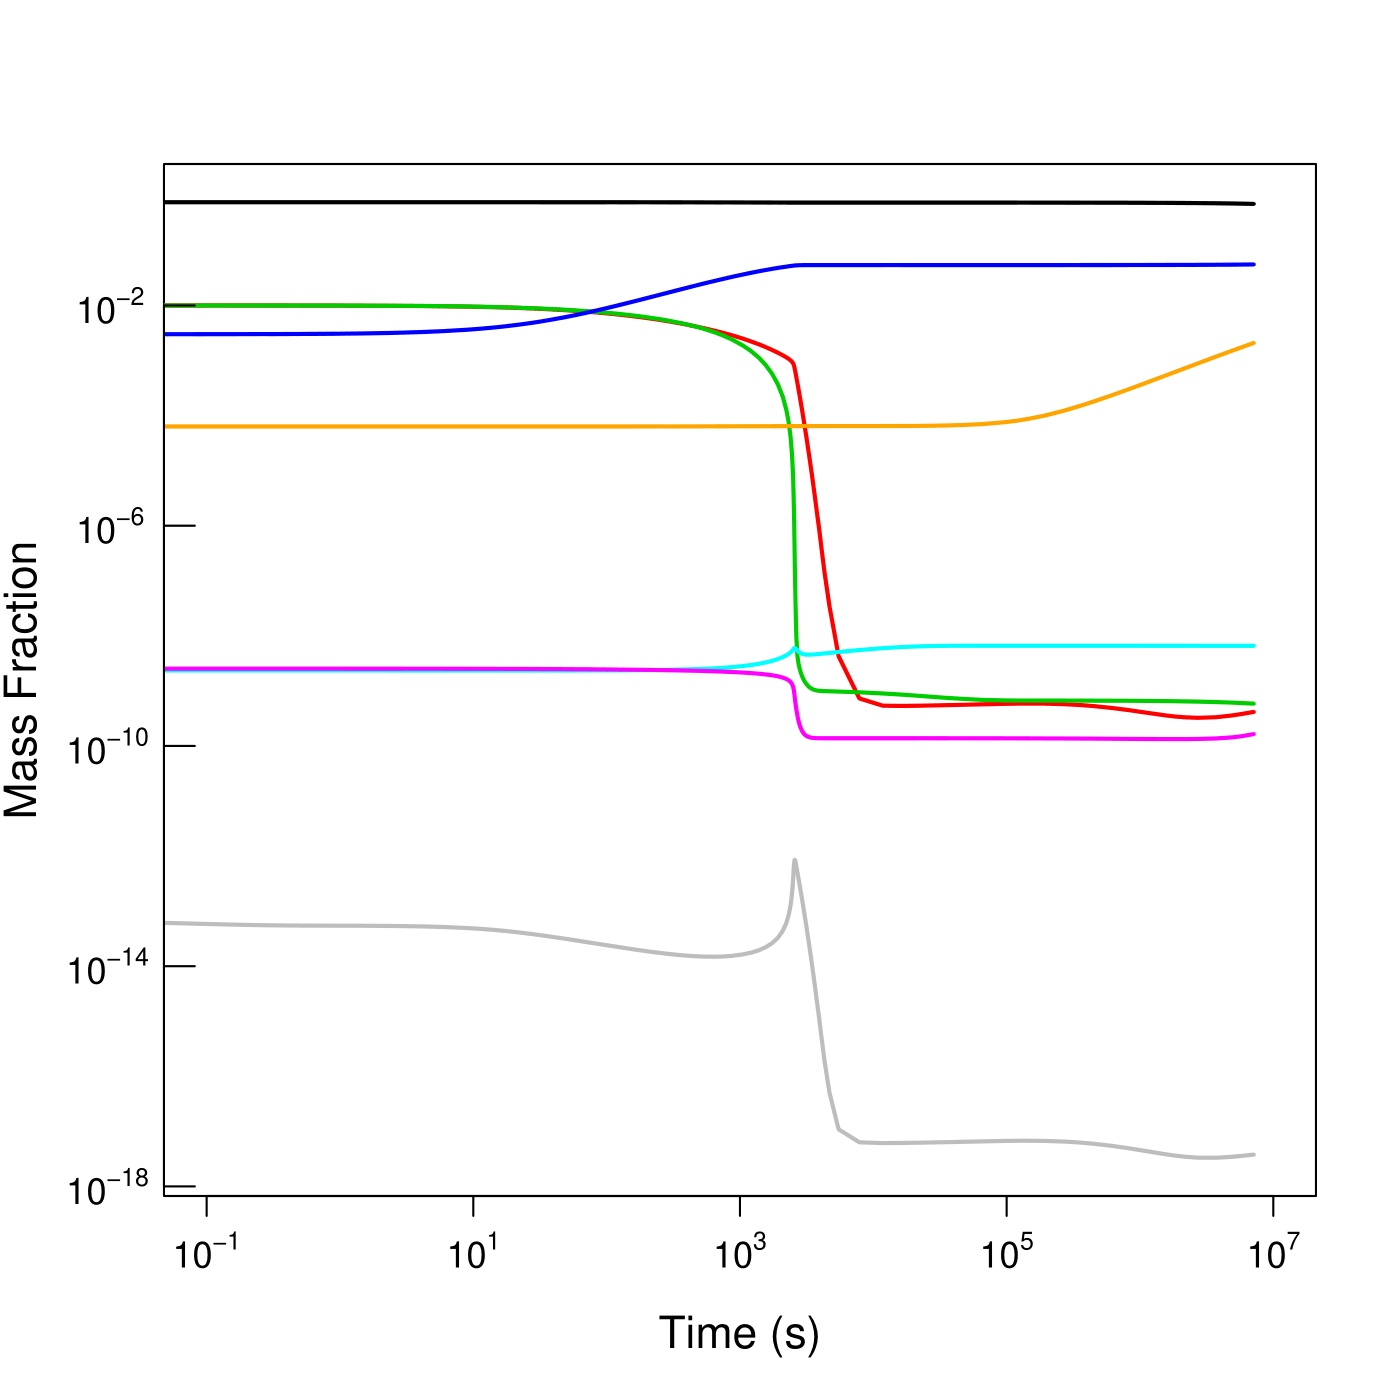
\includegraphics[width=6.5in]{Chapter-3/figs/abund_300MK.png}};
\node at (-1.5,5.6) {$^{4}$He};
\node at (1.8,2) {$^{13}$C};
\node at (0.7,2) {$^{14}$N};
\node at (3,4.75) {$^{16}$O};
\node at (5,3.2) {$^{22}$Ne};
\node at (4,1.0) {$^{87}$Rb};
\node at (4,-0.8) {$^{86}$Sr};
\node at (1.75,-3.5) {$n$};
\node[draw] at (-3,-5) {$T = 300$ MK, $\rho = 10^{3}$ $\mathrm{g}/\mathrm{cm}^{3}$};
\end{tikzpicture}
\caption{\label{fig:abund_evol}The abundance evolution of key nuclei related to the s-process branching at $^{86}$Rb for a single network calculation simulating the conditions during a single AGB thermal pulse. The $T$, $\rho$, and $X_{\mathrm{last}}(^{4}\mathrm{He})$ parameters are 300 MK, $10^{3}$ $\mathrm{g}/\mathrm{cm}^{3}$, and 0.7, respectively, with $X_{\mathrm{init}}(^{4}\mathrm{He}) = 0.75$.}
\end{figure}

\begin{figure}[t]
\centering
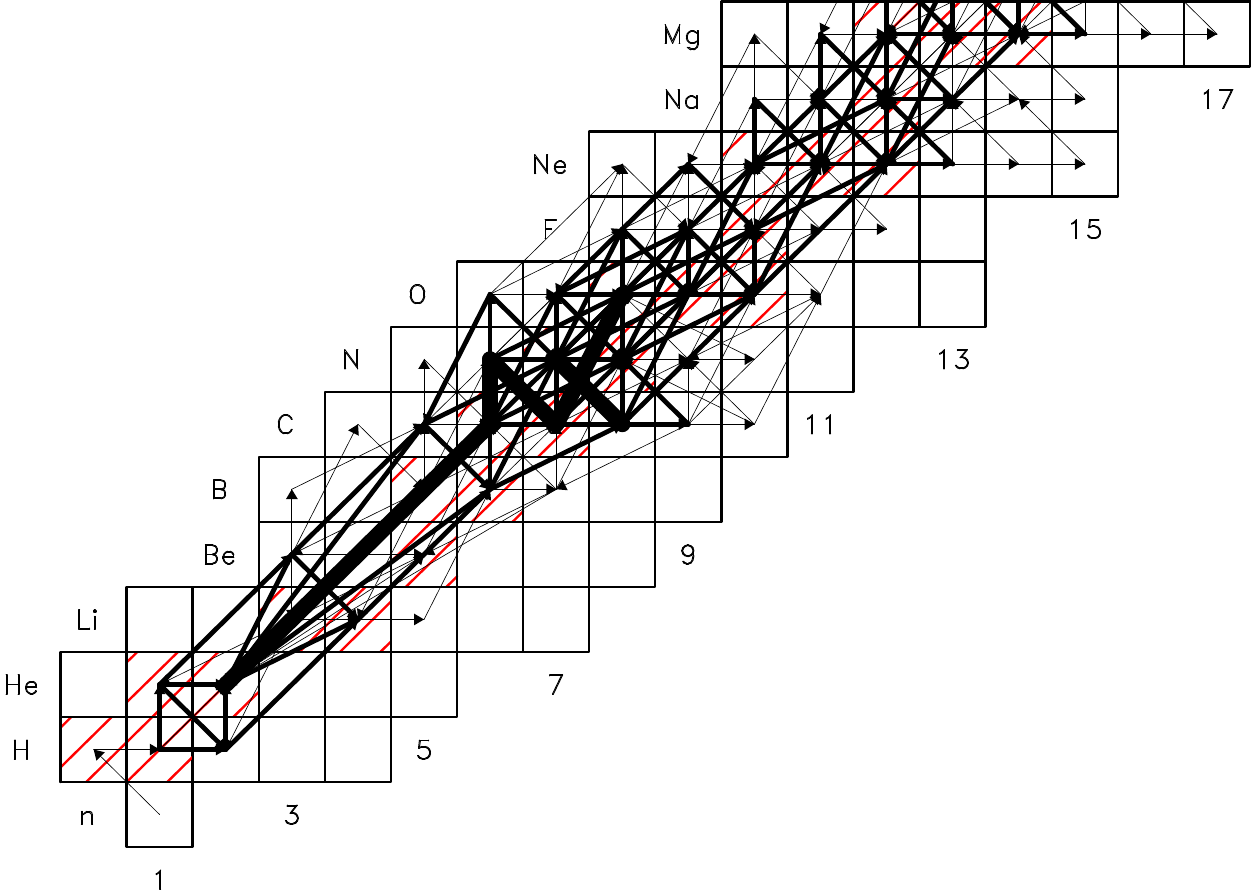
\includegraphics[width=6.5in]{Chapter-3/figs/Flux_300MK_1d3.png}
\caption{\label{fig:Flux}The network flux plot for a single network calculation simulating the conditions during a single AGB thermal pulse. The $T$, $\rho$, and $X_{\mathrm{last}}(^{4}\mathrm{He})$ parameters are 300 MK, $10^{3}$ $\mathrm{g}/\mathrm{cm}^{3}$, and 0.7, respectively, with $X_{\mathrm{init}}(^{4}\mathrm{He}) = 0.75$. The arrow thickness corresponds to the magnitude of the integrated flux from one nucleus to another, with three levels of relative magnitude shown. The reactions with the largest net flux are the triple-$\alpha$ reaction, the $^{13}$C neutron source sequence $^{12}\mathrm{C}(p,\gamma)^{13}\mathrm{N}(\beta^{+}\nu)^{13}\mathrm{C}(\alpha,n)^{16}\mathrm{O}$, and the neutron poison $^{14}\mathrm{N}(n,p)^{14}\mathrm{C}$.}
\end{figure}

% The reaction sequence $^{14}\mathrm{N}(\alpha,\gamma)^{18}\mathrm{F}(\beta^{+}\nu)^{18}\mathrm{O}(\alpha,\gamma)^{22}\mathrm{Ne}$ and the subsequent $^{22}\mathrm{Ne}(\alpha,n)^{25}\mathrm{Mg}$ neutron source are also depicted, albeit to a lesser degree than the $^{13}\mathrm{C}(\alpha,n)^{16}\mathrm{O}$ neutron source.

\subsection{Monte Carlo Procedure}

% Explanation of the Monte Carlo reaction network calculations

\subsection{Measuring Correlations with Mutual Information}

% Explanation of the Spearman, Pearson, and mutual information statistics

\section{Reaction Rate Sensitivities} \label{sec:rate_sensitivities}

\subsection{Correlations}

\begin{figure}[t]
\centering
\begin{subfigure}[b]{0.495\textwidth}
\centering
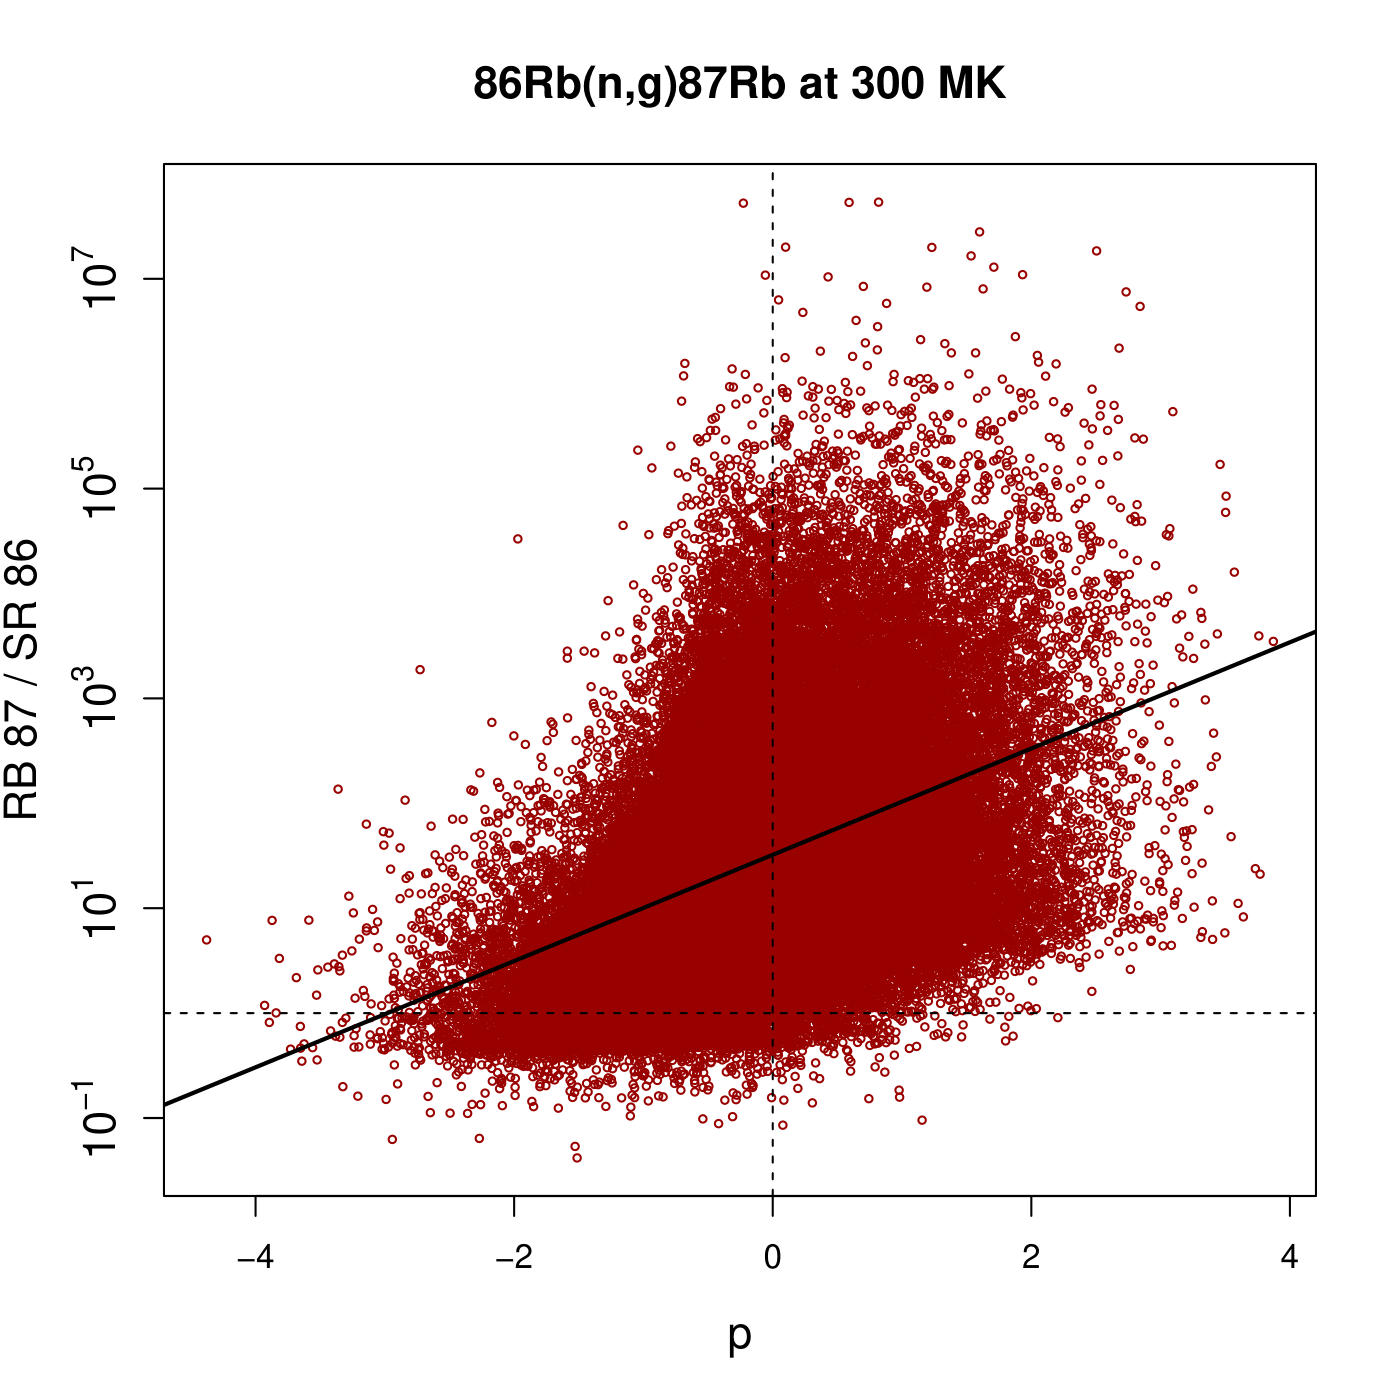
\includegraphics[width=\textwidth]{Chapter-3/figs/CorrRB87SR86_86Rb_n_g_87Rb_300MK.png}  
\end{subfigure}
\hfill
\begin{subfigure}[b]{0.495\textwidth}  
\centering 
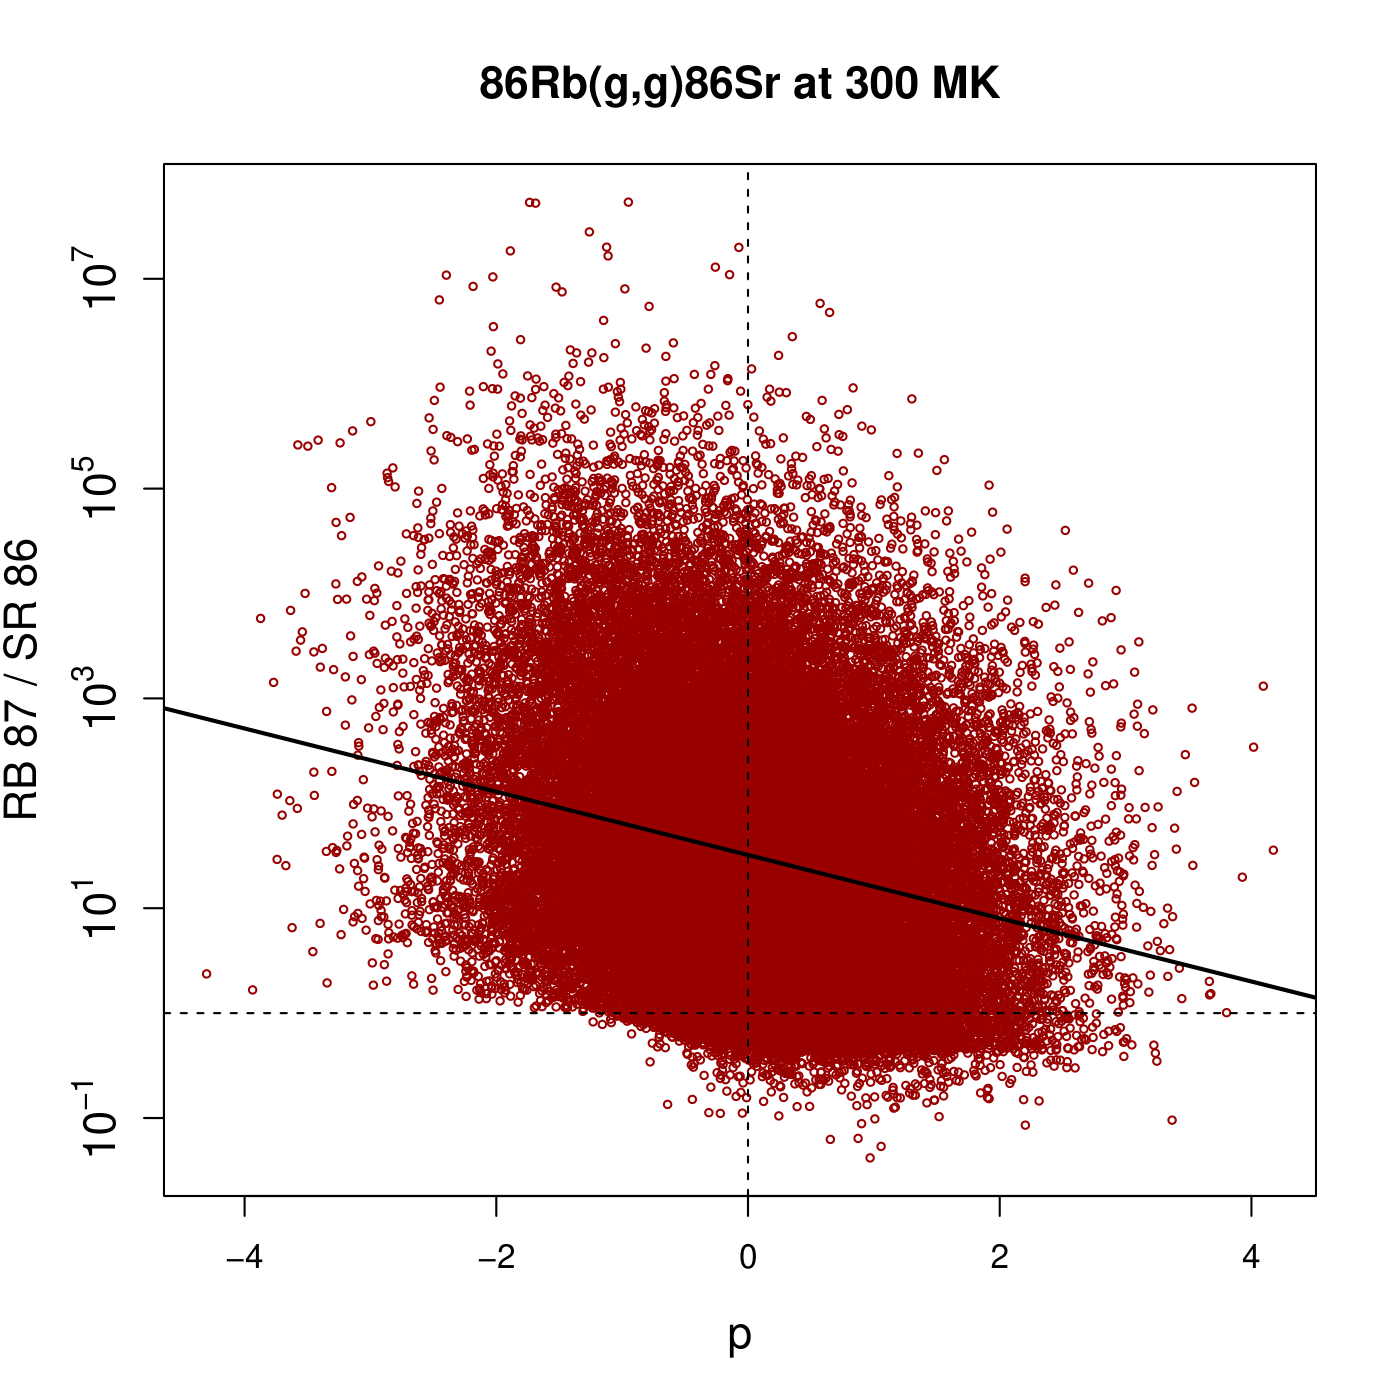
\includegraphics[width=\textwidth]{Chapter-3/figs/CorrRB87SR86_86Rb_g_g_86Sr_300MK.png}
\end{subfigure}
%\vskip\baselineskip
\begin{subfigure}[b]{0.495\textwidth}   
\centering 
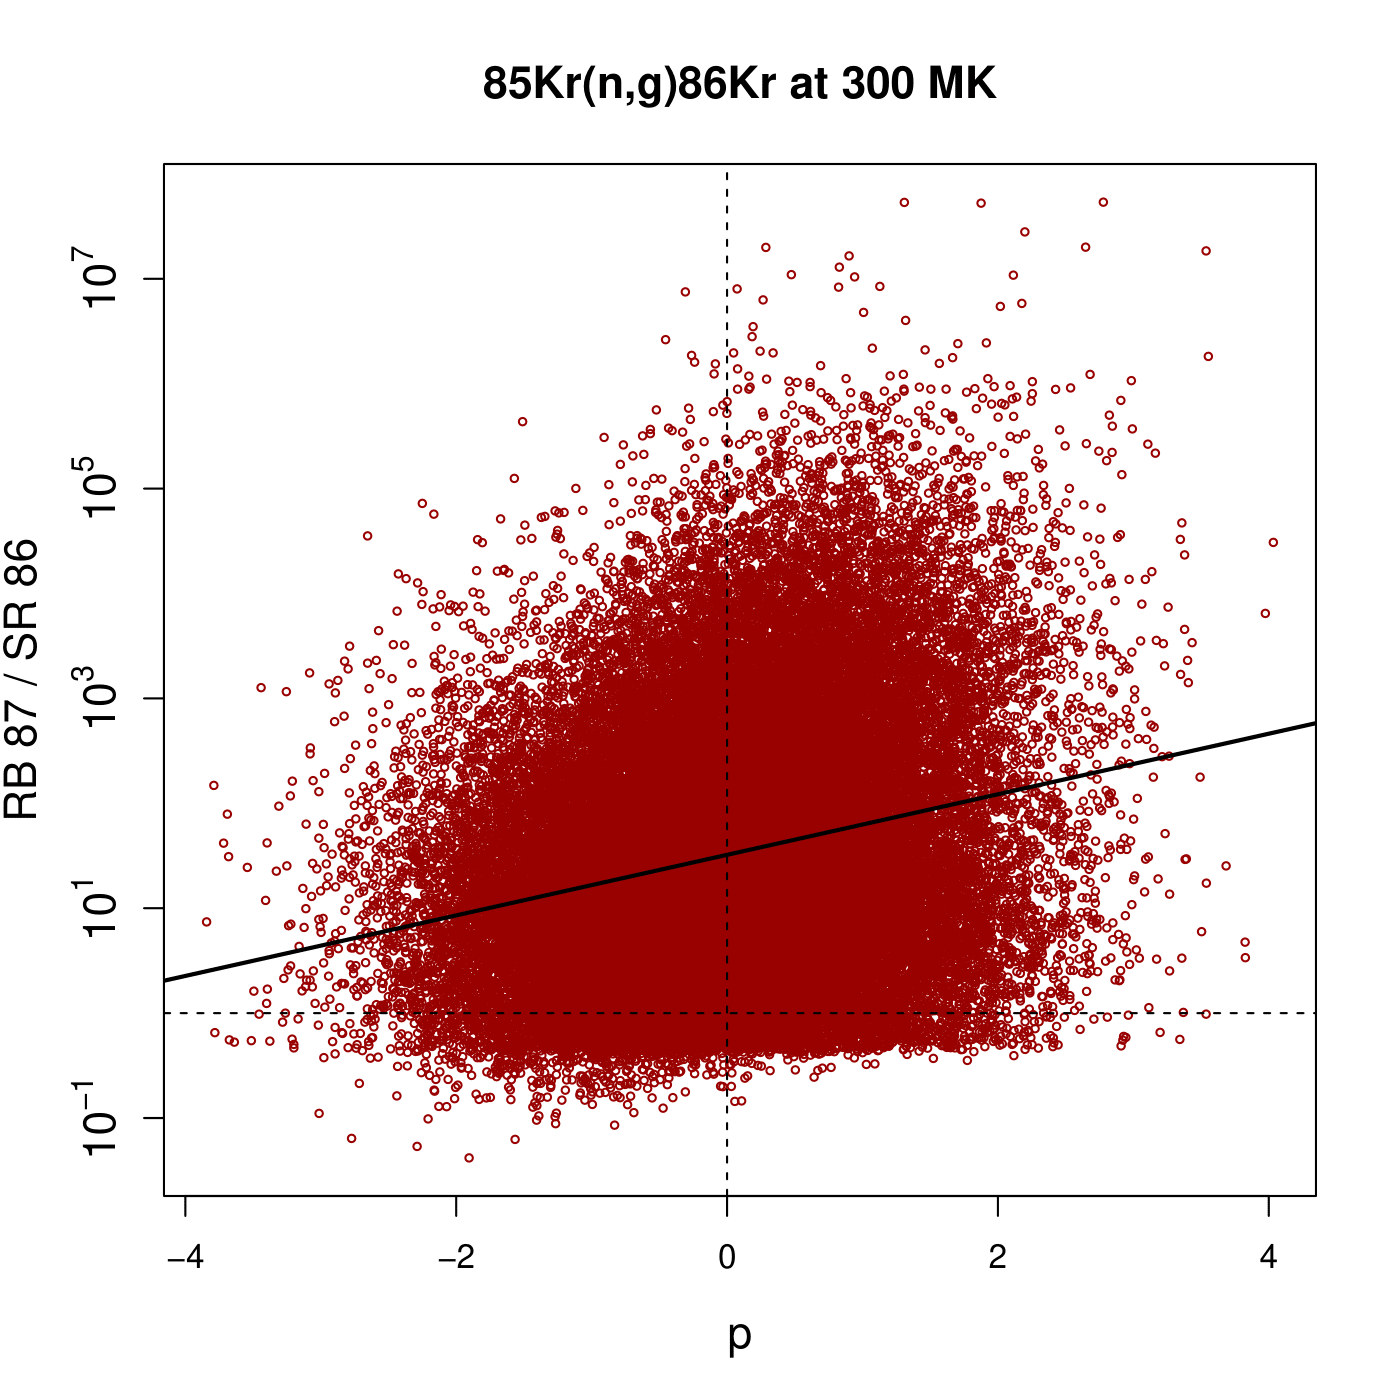
\includegraphics[width=\textwidth]{Chapter-3/figs/CorrRB87SR86_85Kr_n_g_86Kr_300MK.png}
\end{subfigure}
\hfill
\begin{subfigure}[b]{0.495\textwidth}   
\centering 
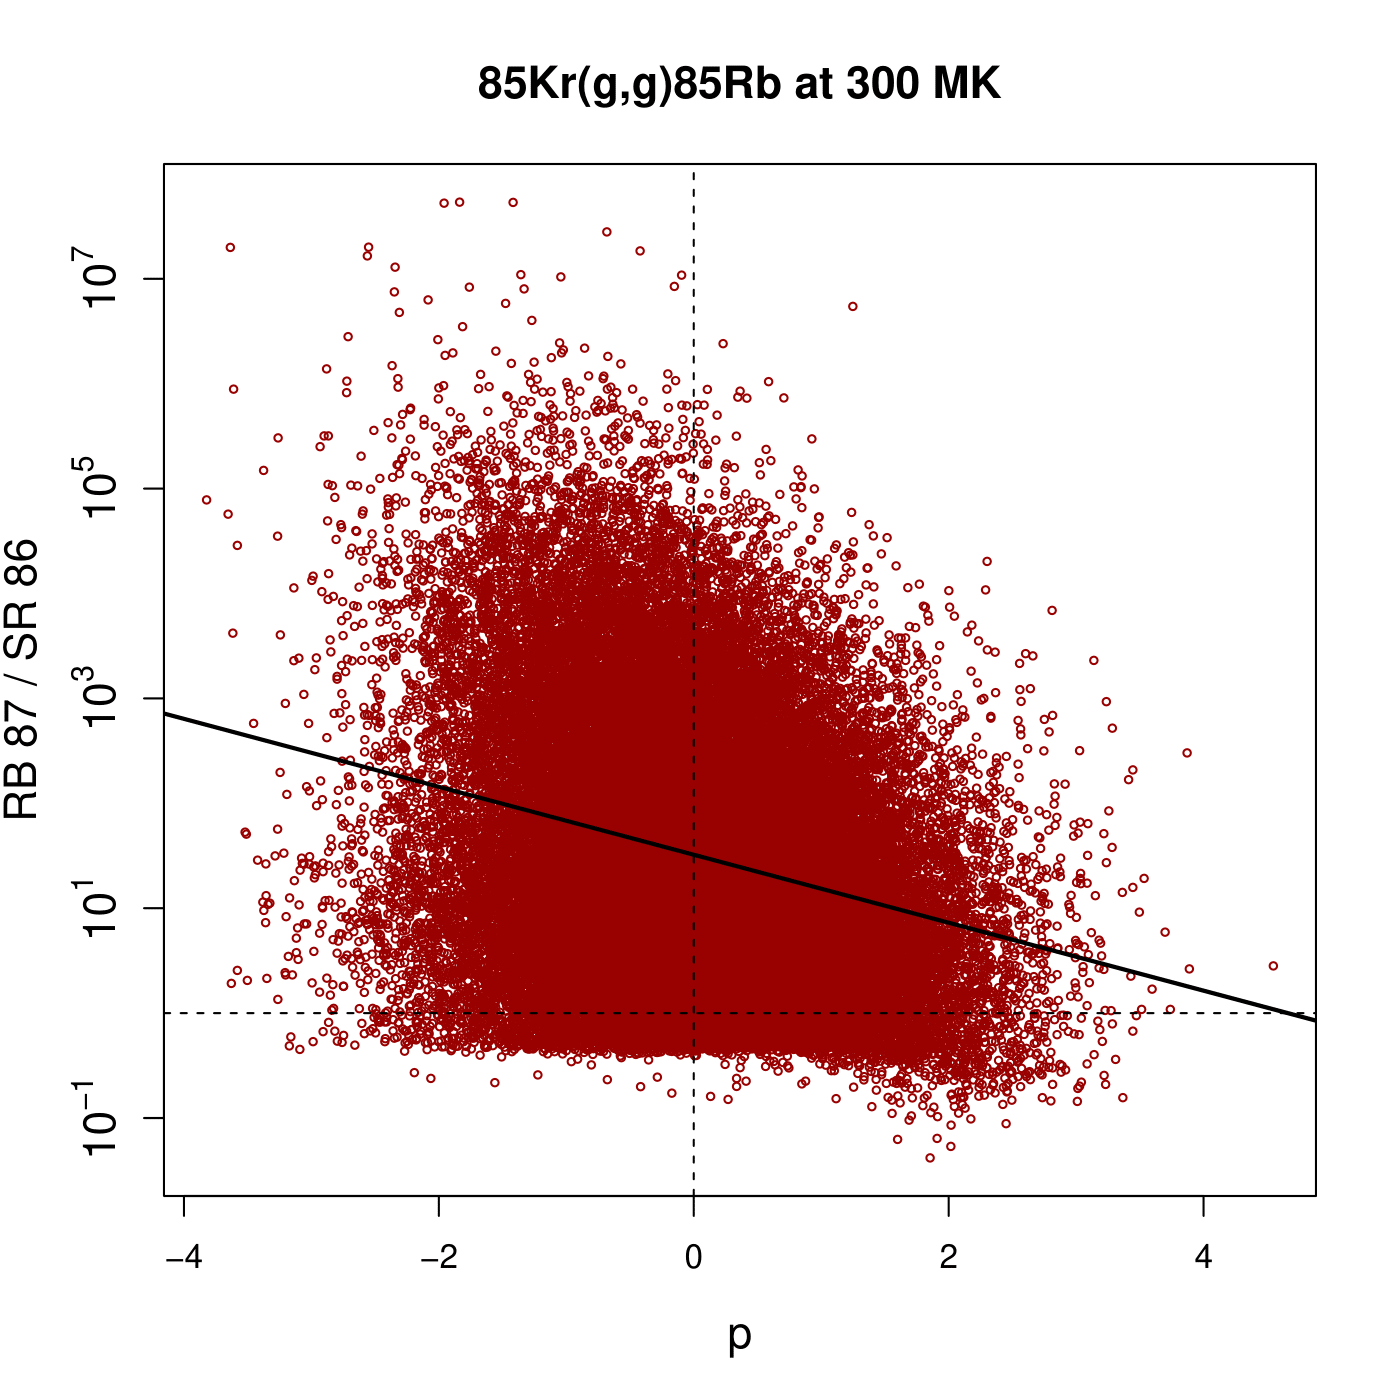
\includegraphics[width=\textwidth]{Chapter-3/figs/CorrRB87SR86_85Kr_g_g_85Rb_300MK.png}
\end{subfigure}
\caption{\label{fig:Correlations_86Rb_Branch}Correlations between the final mass fraction ratio $X(^{87}\mathrm{Rb})/X(^{86}\mathrm{Sr})$ and the relevant reaction rates of the $^{86}$Rb and $^{85}$Kr s-process branchings for $5 \times 10^{4}$ reaction network calculation samples. The $x$-axis is given in terms of the gaussian rate variation factor $p$ (see text). The $T$, $\rho$, and $X_{\mathrm{last}}(^{4}\mathrm{He})$ parameters are 300 MK, $10^{3}$ $\mathrm{g}/\mathrm{cm}^{3}$, and 0.7, respectively, with $X_{\mathrm{init}}(^{4}\mathrm{He}) = 0.75$.} 
\end{figure}

\begin{figure}[t]
\centering
\begin{subfigure}[b]{0.495\textwidth}
\centering
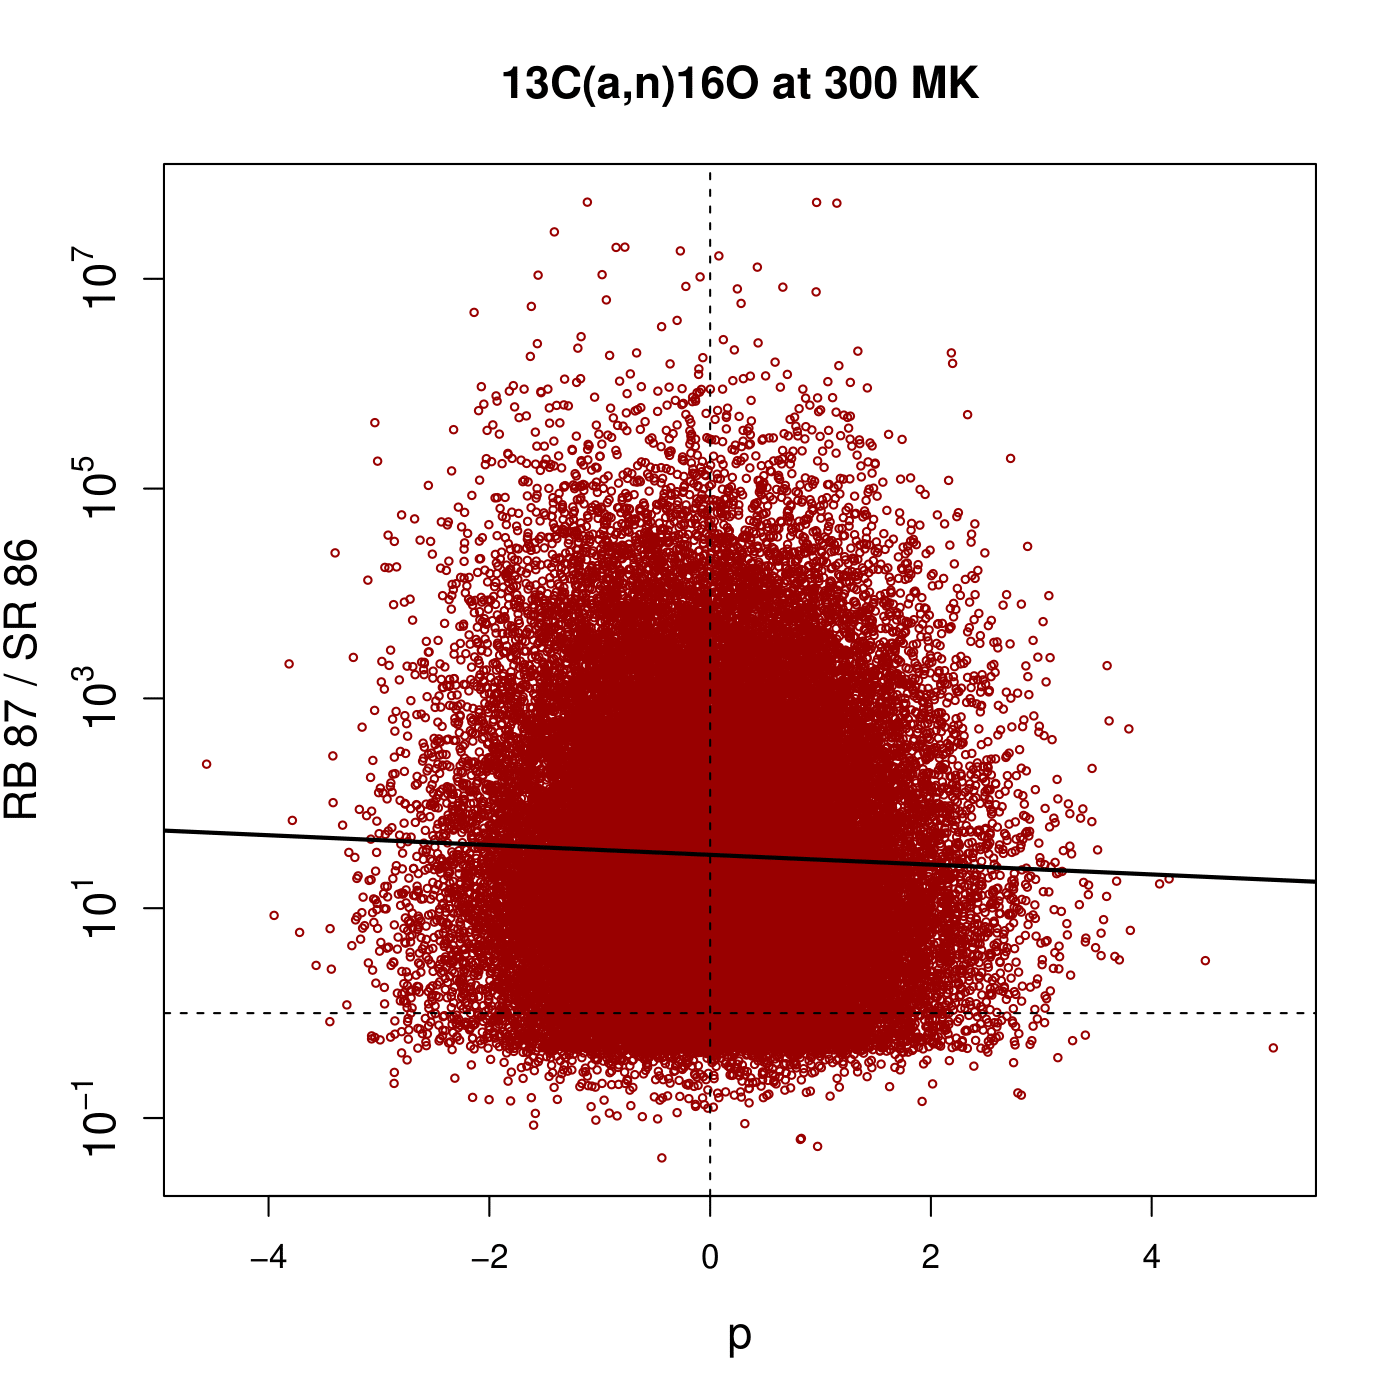
\includegraphics[width=\textwidth]{Chapter-3/figs/CorrRB87SR86_13C_a_n_16O_300MK.png}  
\end{subfigure}
\hfill
\begin{subfigure}[b]{0.495\textwidth}  
\centering 
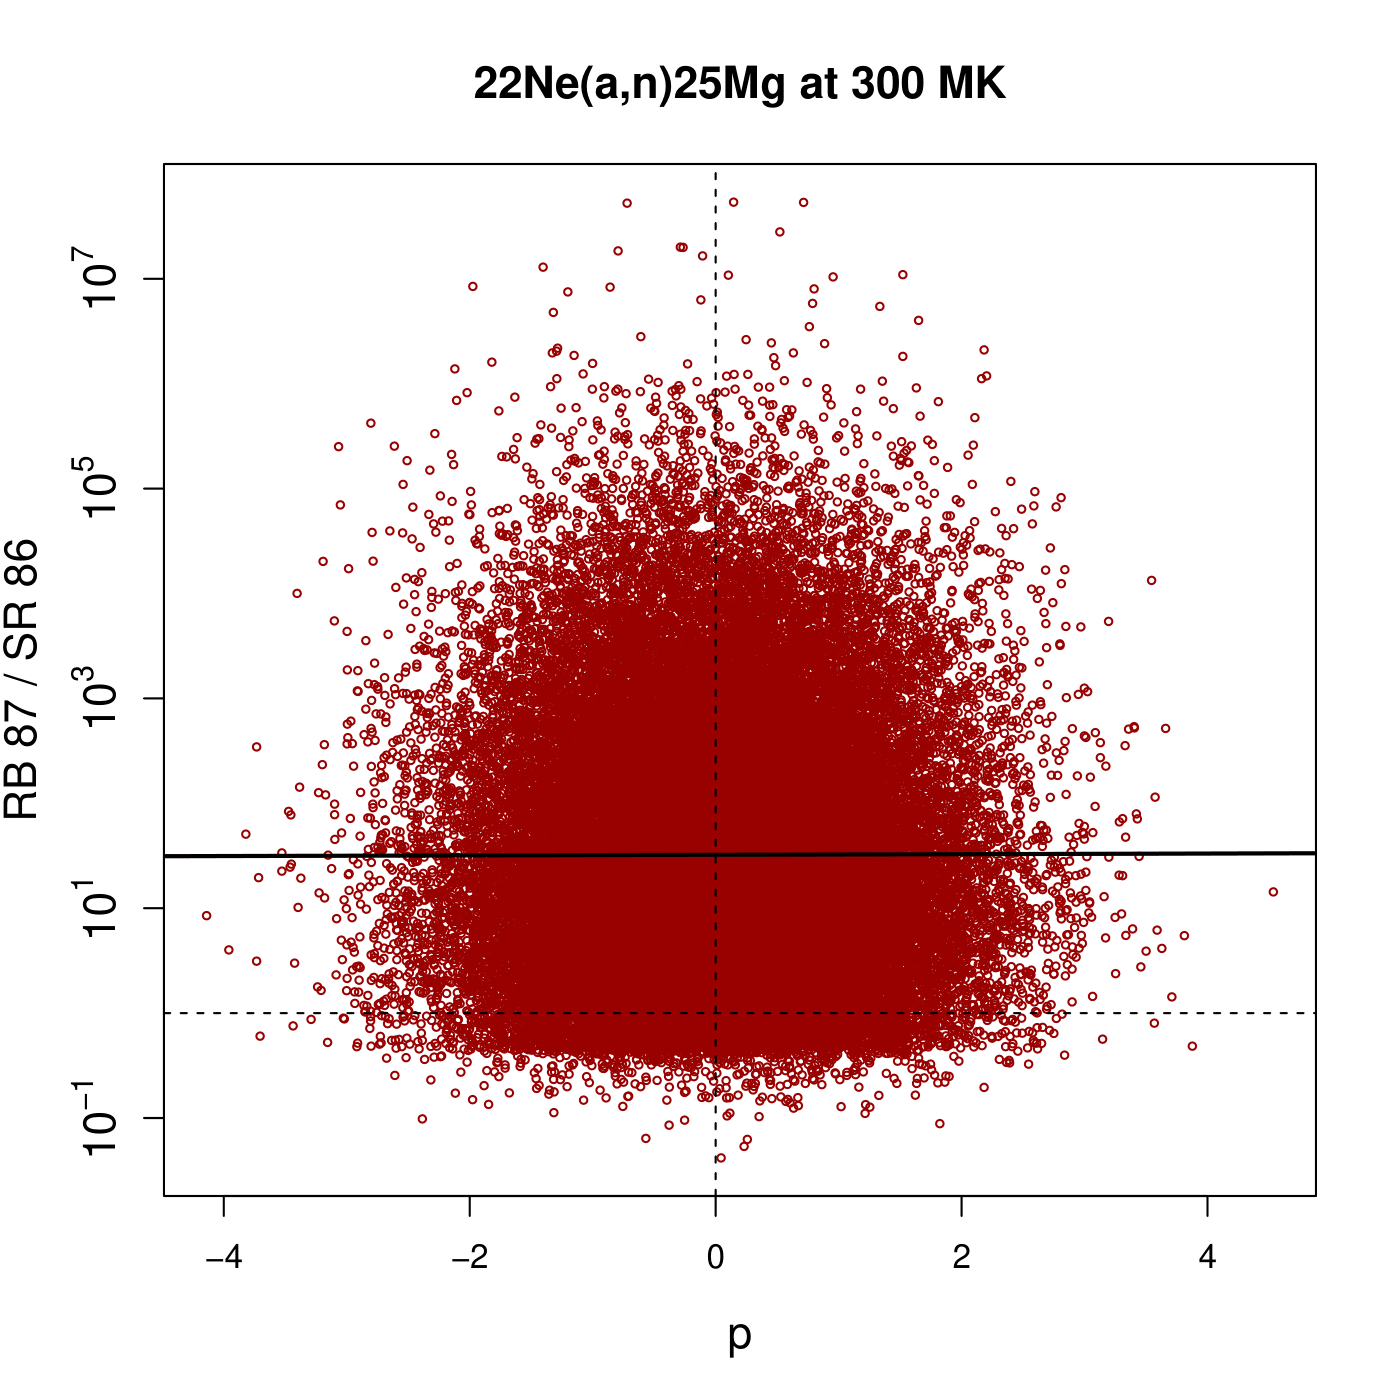
\includegraphics[width=\textwidth]{Chapter-3/figs/CorrRB87SR86_22Ne_a_n_25Mg_300MK.png}
\end{subfigure}
%\vskip\baselineskip
\begin{subfigure}[b]{0.495\textwidth}   
\centering 
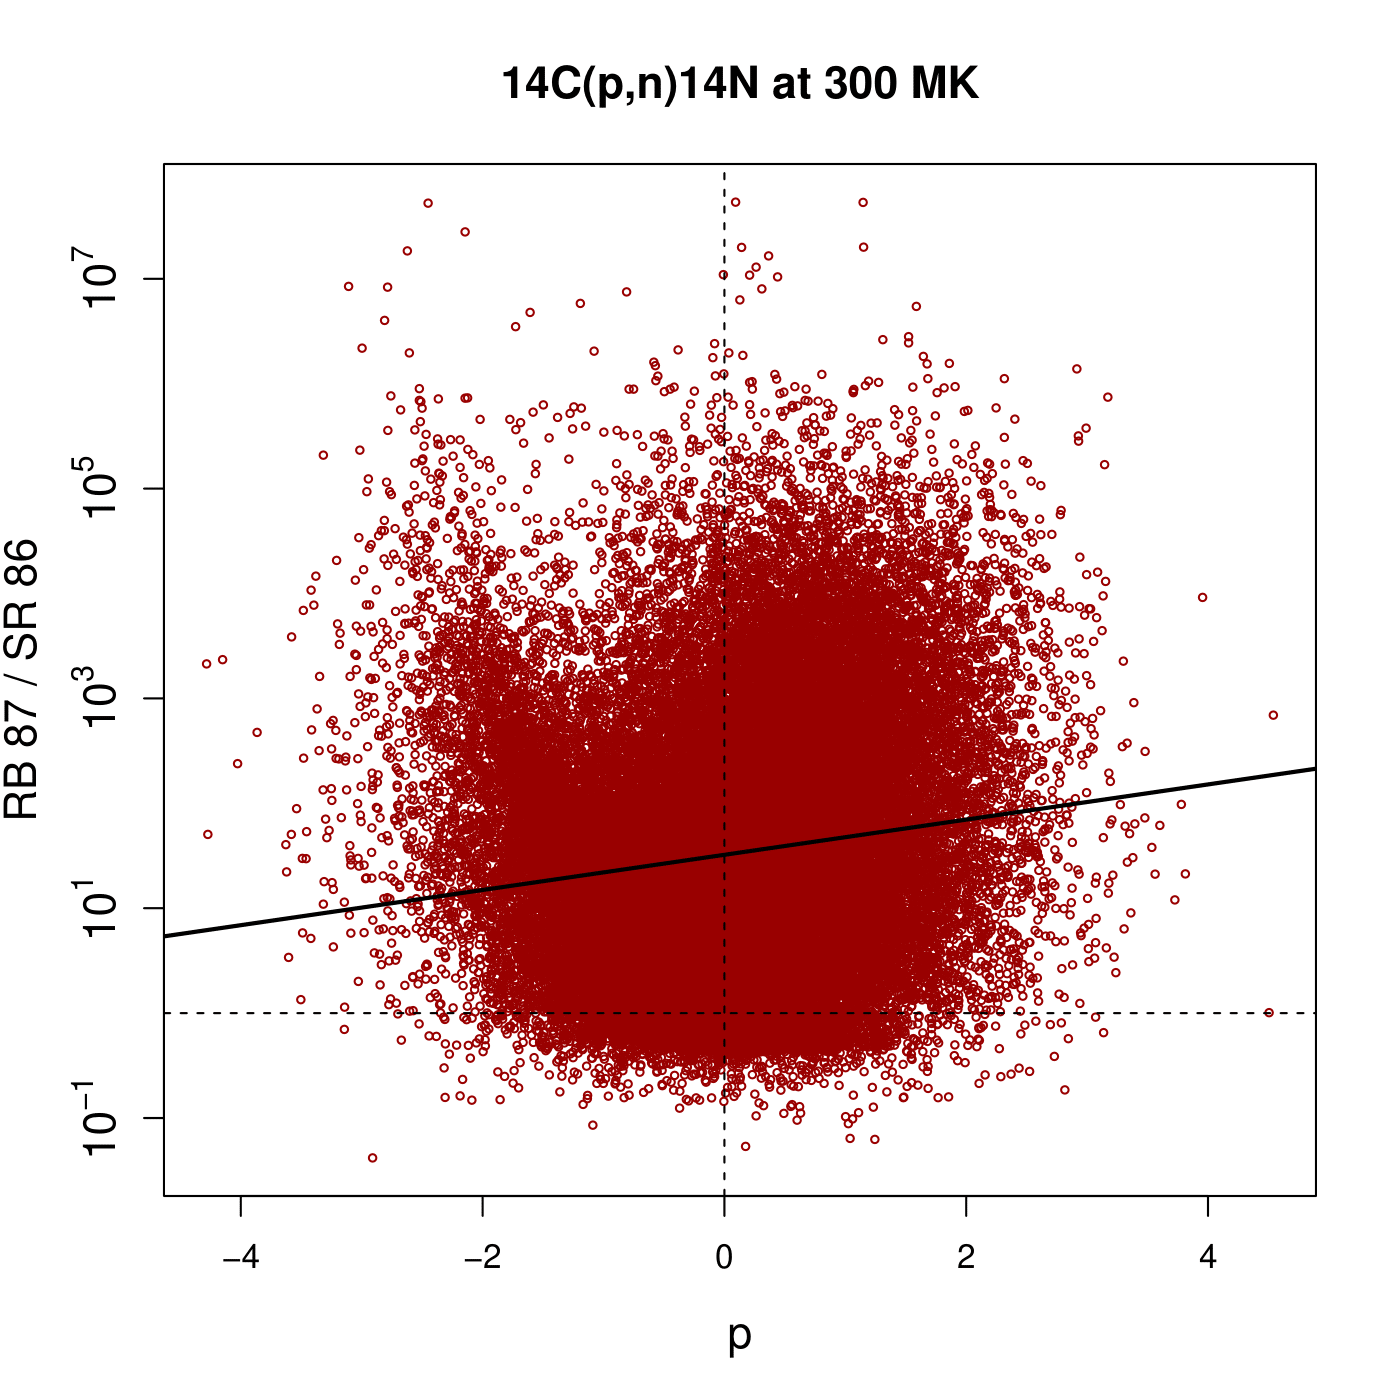
\includegraphics[width=\textwidth]{Chapter-3/figs/CorrRB87SR86_14C_p_n_14N_300MK.png}
\end{subfigure}
\hfill
\begin{subfigure}[b]{0.495\textwidth}   
\centering 
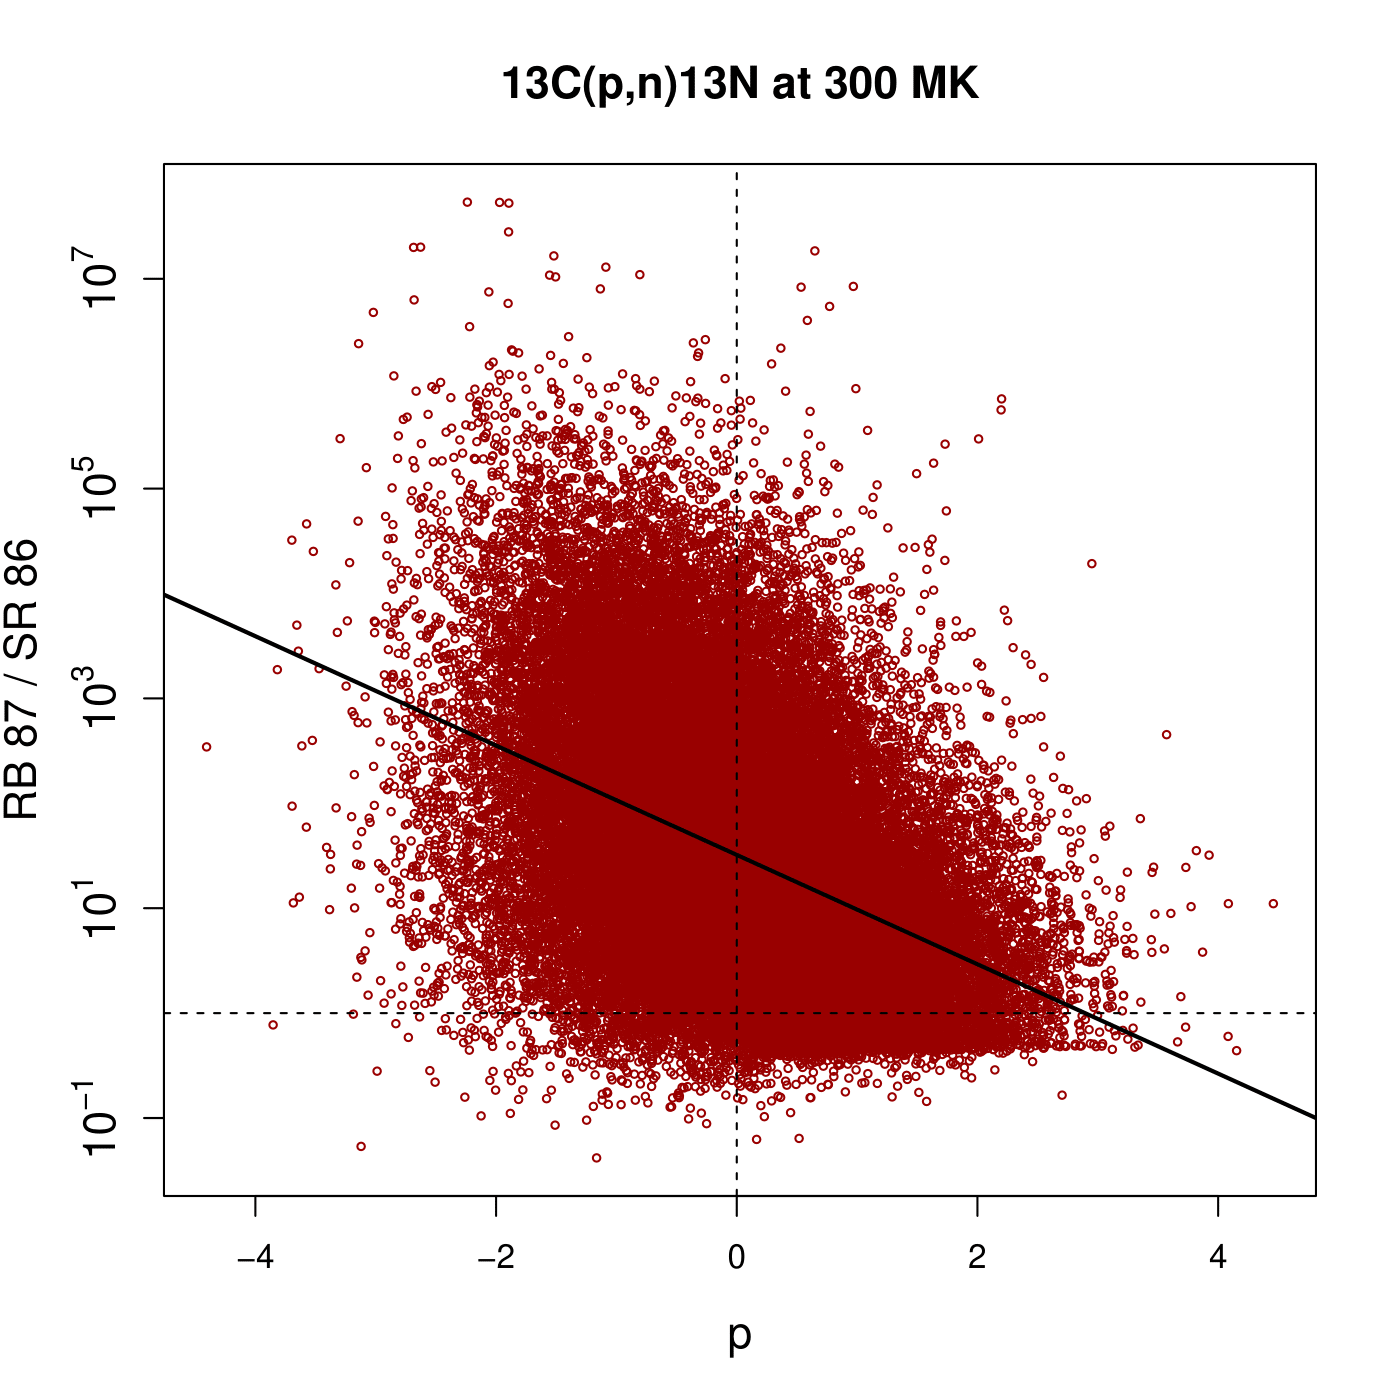
\includegraphics[width=\textwidth]{Chapter-3/figs/CorrRB87SR86_13C_p_n_13N_300MK.png}
\end{subfigure}
\caption{\label{fig:Correlations_neutron_source}Correlations between the final mass fraction ratio $X(^{87}\mathrm{Rb})/X(^{86}\mathrm{Sr})$ and the relevant reaction rates of the s-process neutron sources and neutron poisons for $5 \times 10^{4}$ reaction network calculation samples. The $x$-axis is given in terms of the gaussian rate variation factor $p$ (see text). The $T$, $\rho$, and $X_{\mathrm{last}}(^{4}\mathrm{He})$ parameters are 300 MK, $10^{3}$ $\mathrm{g}/\mathrm{cm}^{3}$, and 0.7, respectively, with $X_{\mathrm{init}}(^{4}\mathrm{He}) = 0.75$.} 
\end{figure}
       
\begin{table}[t]
\centering
\caption{\label{tab:mutual_info}Sensitivities in the $X(^{87}\mathrm{Rb})/X(^{86}\mathrm{Sr})$ and $X(^{87}\mathrm{Rb})/X(^{90}\mathrm{Zr})$ ratios from reaction rate uncertainties, ranked according to mutual information (M.I.). The Spearman correlation coefficient is also provided.}
\begin{tabular}{cccccc}
\hline\midrule
\multicolumn{3}{c}{$X(^{87}\mathrm{Rb})/X(^{86}\mathrm{Sr})$}&
\multicolumn{3}{c}{$X(^{87}\mathrm{Rb})/X(^{90}\mathrm{Zr})$}\\
\cmidrule[0.1pt](l{1.9em}r{.6em}){1-3} \cmidrule[0.1pt](l{1.8em}r{.6em}){4-6}
Reaction&M.I.&Spearman&Reaction&M.I.&Spearman\\ \midrule
$^{86}\mathrm{Rb}(n,\gamma)^{87}\mathrm{Rb}$&0.1967&0.4347
&$^{13}\mathrm{C}(p,n)^{13}\mathrm{N}$&0.1921&-0.4822\\
$^{13}\mathrm{C}(p,n)^{13}\mathrm{N}$&0.1718&-0.4450
&$^{14}\mathrm{N}(n,p)^{14}\mathrm{C}$&0.1331&0.1574\\
$^{14}\mathrm{N}(n,p)^{14}\mathrm{C}$&0.1341&0.1518
&$^{86}\mathrm{Rb}(n,\gamma)^{87}\mathrm{Rb}$&0.1046&0.1405\\
$^{85}\mathrm{Kr}(\beta^{-}\nu)^{85}\mathrm{Rb}$&0.1102&-0.2433
&$^{90}\mathrm{Y}(n,\gamma)^{91}\mathrm{Y}$&0.1039&0.3222\\
$^{86}\mathrm{Rb}(\beta^{-}\nu)^{86}\mathrm{Sr}$&0.1045&-0.2421
&$^{87}\mathrm{Kr}(n,\gamma)^{88}\mathrm{Kr}$&0.0741&-0.2138\\
$^{85}\mathrm{Kr}(n,\gamma)^{86}\mathrm{Kr}$&0.0951&0.2176
&$^{85}\mathrm{Kr}(n,\gamma)^{86}\mathrm{Kr}$&0.0637&0.1973\\
\hline\hline
\end{tabular}
\end{table}

\subsection{The [Rb/Zr] and [Rb/Fe] Ratios}

\begin{figure}[t]
\centering
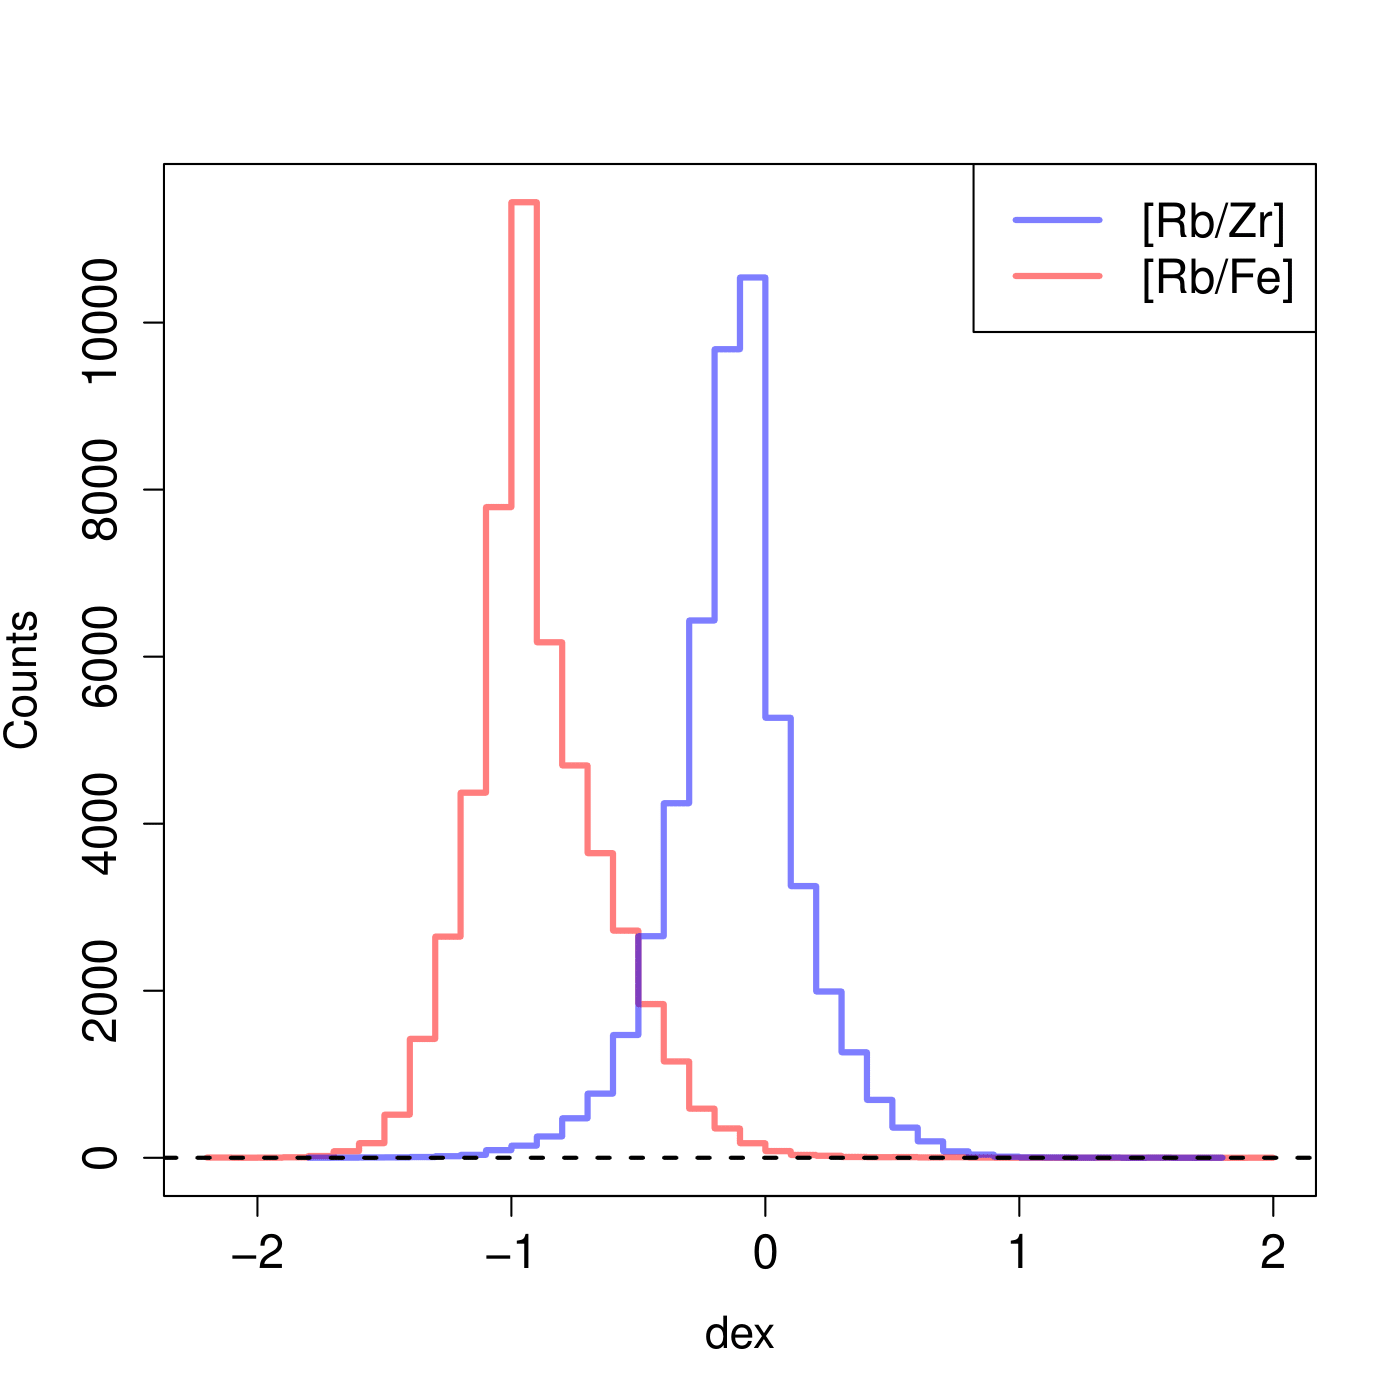
\includegraphics[width=6.5in]{Chapter-3/figs/Hist_Ele_Dex_Ratio_RbZr.png}
\caption{\label{fig:RbZr_Hist}Histogram of the [Rb/Zr] (blue) and [Rb/Fe] (red) abundance ratios from the Monte Carlo reaction network calculation at $T = 300$ MK, $\rho = 10^{3}$ $\mathrm{g}/\mathrm{cm}^{3}$, and $X_{\mathrm{last}}(^{4}\mathrm{He}) = 0.7$, with $X_{\mathrm{init}}(^{4}\mathrm{He}) = 0.75.$}
\end{figure}

\section{The $^{86}\mathrm{\textbf{Rb}}(n,\gamma)^{87}\mathrm{\textbf{Rb}}$ Reaction Rate} \label{sec:86Rb_n_g_rate}

\subsection{Recent Constraint with Nuclear Resonance Fluorescence}
% NRF measurement at HIGS (monoenergetic photons) and $\gamma$ELBE (Bremsstrahlung). Show the PSF and NLD. The NLD is still uncertain. The 86Sr(p,g)87Rb proton-capture reaction would help, and the 86Rb(3He,d)87Rb could be performed too.

%\subsection{The $^{86}\mathrm{\textbf{Kr}}(p,\gamma)^{87}\mathrm{\textbf{Rb}}$ and $^{86}\mathrm{\textbf{Kr}}(^{3}\mathrm{\textbf{He}},d)^{87}\mathrm{\textbf{Rb}}$ Reactions}

% The 87Rb NRF paper mentions 86Kr(p,g)87Rb as a way of reducing the level 

\section{Conclusions}

